\chapter{Introduction}

\section{Project Aims and Motivation}

The project aims to build a ball perception system, to be a component of a complete football playing  robot. The system will be made for the MiRo robot which has forward-facing stereo cameras that can be used for ball detection, however its limited processing power is a factor that will limit the techniques that can be used to achieve this. 

There are three key problems that the project will tackle; measuring ball position, measuring ball velocity and predicting ball trajectory. 

The ball position can be detected using the cameras, however it must be measured in world space to be useful for decision making. Therefore an world space conversion is required as well as a computer vision algorithm. This algorithm should be reasonably accurate while being efficient enough to run in real time.

The ball velocity can be estimated using recent observed ball positions, however noise in these observations should be expected. 

A prediction for the ball trajectory is necessary for planning a route to intercept the ball. 

\section{RoboCup}

In 1993 a group of Japanese researchers decided to start a robot football league, and after receiving great support from researchers across the world the league was made international, and named the Robot World Cup initiative, or RoboCup for short. Four years later the first ever RoboCup competition was held in Japan. 

The tournament is held annually, having teams compete in 5 types of football leagues: humanoid, standard platform, middle size, small size and simulation. RoboCup also has some leagues for problems outside of football: rescue, home and industrial.

Since its conception, the goal of RoboCup has been the following: "By the middle of the 21st century, a team of fully autonomous humanoid robot soccer players shall win a soccer game, complying with the official rules of FIFA, against the winner of the most recent World Cup." This makes RoboCup a landmark project - the accomplishment of this goal would be a landmark in the history of mankind. RoboCup is also a standard problem - technologies developed to achieve its goal will be useful in the area of AI and robotics.

\section{MiRo}

MiRo is an animal-like robot developed by Consequential Robotics for education and research purposes. MiRo excels in its social behaviour, with numerous touch sensors around its body and 11 degrees of freedom allowing believable animal-like movement. However MiRo also has all of the necessary features to be able to play football. 

It has stereo cameras able to capture images in 720p. Each camera has a 120\degree horizontal field of view with an overlap slightly over 60\degree meaning that they have a combined horizontal field of view of nearly 120\degree. MiRo can move using a differential drive platform that gives a maximum speed of 400mm/sec. The biggest limitation of the robot is its onboard computer, a Raspberry Pi 3B+ containing a 1.4GHz 64-bit quad-core processor. 

\begin{figure}[H]
    \centering
    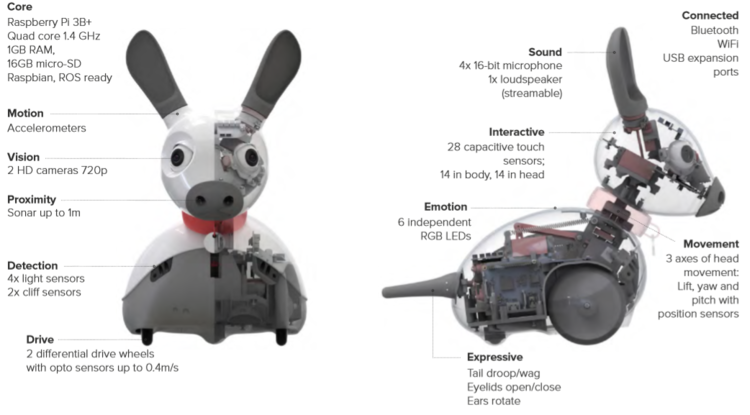
\includegraphics[width=12cm]{images/miro-specs.png}
    \caption{Full specifications of the MiRo robot}
    \label{fig:miro specs}
    Source: \url{https://www.miro-e.com/robot}
\end{figure}

\section{Computer Vision}

Computer vision is a field of artificial intelligence which is concerned with the extraction of information from digital images. It has many sub-domains, such as object recognition or identification, but the perception of a ball in an image falls into object detection. 

Object detection is a technique that involves finding instances of a specific class in an image. The various methods of object detection can be classified into two approaches, neural and non-neural. For non-neural techniques, a feature vector must be obtained from the image, which must then be evaluated by a classifier. Neural techniques are able to do object detection without needing to defining features. They can be more powerful than non-neural methods, however they are more computationally expensive to train and to run.

\section{Motion Planning}

Motion planning is the problem of finding a valid path so that a robot moves from some initial position to a goal, avoiding any obstacles along the way. Bruce\cite{Bruce2006} outlines some different categories of dynamics in motion planning problems. The first is agent and domain dynamics. Agent dynamics refers to the effects of physics on the agent itself, for example the kinematic constraints on the motion of the agent. Conversely domain dynamics involves changes to the problem instance over time, for example changes in the environment or goal state.

Another way of categorising dynamics is into predictable and unpredictable dynamics. Predictable dynamics involve variables that can accurately be modelled, such as using the physics of acceleration and velocity. Unpredictable dynamics relate to aspects that cannot be modelled, for example actions taken by other agents, humans or random events.

Bruce also categorises dynamics into local and global dynamics, describing that effect the local and non-local areas to the agent respectively.

This project only aims to tackle the predictable domain dynamics of building an accurate model for the movement of the goal state (i.e. the ball).

\section{Overview of the Report}

Chapter \ref{chapter: 2} gives an overview of relevant work that has already been completed, primarily by teams competing in previous iterations of RoboCup. This includes methods for estimating ball position and velocity, as well as predicting ball trajectory. 

Chapter \ref{chapter: 3} outlines the objectives that the project aims to achieve, elaborating on each point and giving detail on how each part of the system will be evaluated. 

Chapter \ref{chapter: 4} provides detail on the design of the project. This starts with a description of the tools that are used to develop the system, and then goes on to break down and justify each decision that had to be made regarding the design of each part of the system. 

Chapter \ref{chapter: 5} goes into detail about the notable algorithms that were developed, including the circular Hough transform, support-vector machine classifier and image space to world space conversion. 

Chapter \ref{chapter: 6} presents the results showing the performance of each part of the system, and discusses how successfully each objective was met as well as suggesting some areas for which future work on the system could be completed. 

Chapter \ref{chapter: 7} brings the project to a close, summarising what has been achieved.